% Copyright 2004 by Till Tantau <tantau@users.sourceforge.net>.
%
% In principle, this file can be redistributed and/or modified under
% the terms of the GNU Public License, version 2.
%
% However, this file is supposed to be a template to be modified
% for your own needs. For this reason, if you use this file as a
% template and not specifically distribute it as part of a another
% package/program, I grant the extra permission to freely copy and
% modify this file as you see fit and even to delete this copyright
% notice. 

\documentclass[handout]{beamer}
\usepackage{boondox-cal}
\usepackage{tikz}
\usepackage{multirow}
\usepackage{pgfpages}
%\usepackage{handoutWithNotes}
%
%  Load other packages you may need here
% 
% \pgfpagesuselayout{4 on 1}[a4paper,landscape,border shrink=5mm
%\pgfpagesuselayout{4 on 1}[a4paper,landscape,border shrink=5mm]
%
\usetikzlibrary{bayesnet}
\usepackage{kotex}
\usepackage{amsfonts}
\usepackage{subcaption}
\captionsetup{compatibility=false}
\usepackage{amssymb}
\newcommand{\E}{\mathbb{E}}
\usepackage{amsthm}
\usepackage{latexsym,amsmath}
\usepackage{graphicx}
\usepackage{pgfplots}
\usepackage{afterpage}
\usepackage[ ]{algorithm2e}
\usepackage{bm}
\newcommand{\R}{\mathbb{R}}
\DeclareMathOperator*{\argmin}{arg\,min}
% There are many different themes available for Beamer. A comprehensive
% list with examples is given here:
% http://deic.uab.es/~iblanes/beamer_gallery/index_by_theme.html
% You can uncomment the themes below if you would like to use a different
% one:
%\usetheme{AnnArbor}
%\usetheme{Antibes}
%\usetheme{Bergen}
%\usetheme{Berkeley}
%\usetheme{Berlin}
%\usetheme{Boadilla}
%\usetheme{boxes}
%\usetheme{CambridgeUS}
%\usetheme{Copenhagen}
%\usetheme{Darmstadt}
%\usetheme{default}
%\usetheme{Frankfurt}
%\usetheme{Goettingen}
%\usetheme{Hannover}
%\usetheme{Ilmenau}
%\usetheme{JuanLesPins}
%\usetheme{Luebeck}
\usetheme{Madrid}
%\usetheme{Malmoe}
%\usetheme{Marburg}
%\usetheme{Montpellier}
%\usetheme{PaloAlto}
%\usetheme{Pittsburgh}
%\usetheme{Rochester}
%\usetheme{Singapore}
%\usetheme{Szeged}
%\usetheme{Warsaw}

\title{Density Ratio Estimation in Variational Bayesian Machine Learning}
\thispagestyle{empty}
\addtocounter{framenumber}{-1}	
% A subtitle is optional and this may be deleted
%\subtitle{Optional Subtitle}

\author{Alexander Lam}

% - Give the names in the same order as the appear in the paper.
% - Use the \inst{?} command only if the authors have different
%   affiliation.

\institute[UNSW] % (optional, but mostly needed)
{
  Supervised by Prof. Scott Sisson and Doctor Edwin Bonilla
  }
% - Use the \inst command only if there are several affiliations.
% - Keep it simple, no one is interested in your street address.

\date{Statistics Honours, 2018}
% - Either use conference name or its abbreviation.
% - Not really informative to the audience, more for people (including
%   yourself) who are reading the slides online

\subject{Statistics}
% This is only inserted into the PDF information catalog. Can be left
% out. 

% If you have a file called "university-logo-filename.xxx", where xxx
% is a graphic format that can be processed by latex or pdflatex,
% resp., then you can add a logo as follows:

% \pgfdeclareimage[height=0.5cm]{university-logo}{university-logo-filename}
% \logo{\pgfuseimage{university-logo}}

% Delete this, if you do not want the table of contents to pop up at
% the beginning of each subsection:
%\AtBeginSection[]
%{
%  \begin{frame}<beamer>{Outline}
%    \tableofcontents[currentsection,currentsubsection]
%  \end{frame}
%}

% Let's get started
\begin{document}

\begin{frame}
  \titlepage
\end{frame}

\begin{frame}{Outline}
  \tableofcontents
  % You might wish to add the option [pausesections]
\end{frame}

% Section and subsections will appear in the presentation overview
% and table of contents.
\section{Background Information}

\subsection{Neural Networks}

\begin{frame}{Neural Networks}{Overall Structure}
  \begin{itemize}
  \item {
  	Objective is to approximate a function $f^*$ using mapping with parameters $\bm{\Theta}$: $\textbf{f}_{\bm{\Theta}}(\bm{x})$.  
  }
  \vspace{0.1cm}
  \item {
  	Universal Approximation Theorem states a neural network can\textbf{ approximate (almost) any function} if it is complex enough.
  }
  \vspace{0.1cm}
  \item {
    Each node output is a transformed, weighted sum of previous node outputs.
  }
  \end{itemize}
  \begin{figure}[h!]
  \scalebox{0.7}{
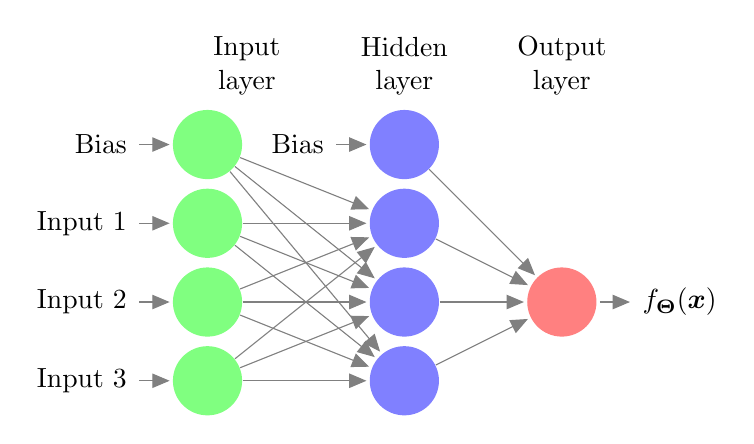
\begin{tikzpicture}[shorten >=1pt,->,draw=black!50, node distance=2.0cm]
    \tikzstyle{every pin edge}=[<-,shorten <=1pt]
    \tikzstyle{neuron}=[circle,fill=black!25,minimum size=25pt,inner sep=0pt]
    \tikzstyle{input neuron}=[neuron, fill=green!50];
    \tikzstyle{output neuron}=[neuron, fill=red!50];
    \tikzstyle{hidden neuron}=[neuron, fill=blue!50];
    \tikzstyle{annot} = [text width=4em, text centered]
    
	\node[input neuron, pin=left:Bias] (I-0) at (-2,0) {};
    % Draw the input layer nodes
    \foreach \name / \y in {1,...,3}
    % This is the same as writing \foreach \name / \y in {1/1,2/2,3/3,4/4}
        \node[input neuron, pin=left:Input \y] (I-\name) at (-2,-\y) {};

 \path[yshift=0cm]
            node[hidden neuron, pin=left:Bias] (H-0) at (0.5cm,0) {};
    % Draw the hidden layer nodes
    \foreach \name / \y in {1,...,3}
        \path[yshift=0cm]
            node[hidden neuron] (H-\name) at (0.5cm,-\y) {};

    % Draw the output layer node
	\path[yshift=1cm]    
    node[output neuron,pin={[pin edge={->}]right:$f_{\bm{\Theta}}(\bm{x})$}, right of=H-2] (O) {};

    % Connect every node in the input layer with every node in the
    % hidden layer.
    \foreach \source in {0,...,3}
        \foreach \dest in {1,...,3}
            \path (I-\source) edge (H-\dest);

    % Connect every node in the hidden layer with the output layer
    \foreach \source in {0,...,3}
        \path (H-\source) edge (O);

    % Annotate the layers
    \node[annot,above of=H-0, node distance=1cm] (hl) {Hidden layer};
    \node[annot,left of=hl] {Input layer};
    \node[annot,right of=hl] {Output layer};
\end{tikzpicture}
}
\end{figure}

\end{frame}
\begin{frame}{Neural Networks}{Individual Node}
\begin{figure}
\scalebox{0.8}{
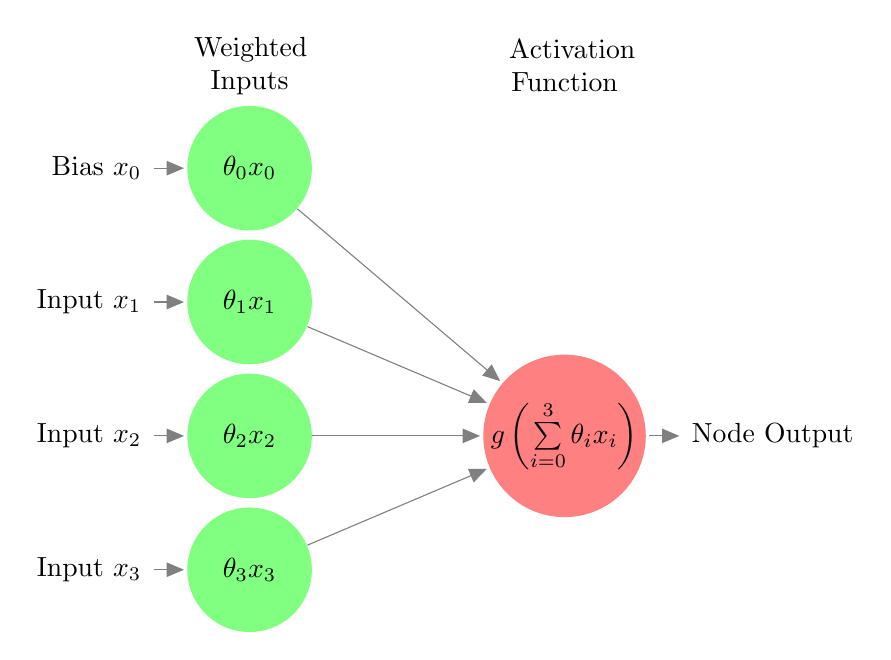
\begin{tikzpicture}[shorten >=1pt,->,draw=black!50, node distance=2.5cm]
    \tikzstyle{every pin edge}=[<-,shorten <=1pt]
    \tikzstyle{neuron}=[circle,fill=black!25,minimum size=45pt,inner sep=0pt]
    \tikzstyle{input neuron}=[neuron, fill=green!50];
    \tikzstyle{output neuron}=[neuron, fill=red!50];
    \tikzstyle{hidden neuron}=[neuron, fill=blue!50];
    \tikzstyle{annot} = [text width=4em, text centered]

    % Draw the input layer nodes
 %   \foreach \name / \y in {0,...,3}
    % This is the same as writing \foreach \name / \y in {1/1,2/2,3/3,4/4}
        \node[input neuron, pin=left:Bias $x_0$] (I-0) at (0,-0) {$\theta_0 x_0$};
	\foreach \name / \y in {1,...,3}
    % This is the same as writing \foreach \name / \y in {1/1,2/2,3/3,4/4}
        \node[input neuron, pin=left:Input $x_{\y}$] (I-\name) at (0,-1.7*\y) {$\theta_{\y}x_\y$};
    % Draw the hidden layer nodes
    %\foreach \name / \y in {1,...,5}
     %   \path[yshift=0.5cm]
      %      node[hidden neuron] (H-\name) at (\layersep,-\y cm) {};

    % Draw the output layer node
    \node[output neuron,pin={[pin edge={->}]right:Node Output}, right of=I-2, node distance=4cm] (O) {$g\left(\sum\limits^3_{i=0}\theta_ix_i\right)$};

    % Connect every node in the input layer with every node in the
    % hidden layer.
   % \foreach \source in {1,...,4}
    %    \foreach \dest in {1,...,5}
     %       \path (I-\source) edge (H-\dest);

    % Connect every node in the hidden layer with the output layer
    \foreach \source in {0,...,3}
        \path (I-\source) edge (O);

    % Annotate the layers
%    \node[annot,above of=H-1, node distance=1cm] (hl) {Hidden layer};
    \node[annot,above of=I-0, node distance=1.3cm](il) {Weighted Inputs};
    \node[annot,right of=il, node distance=4cm] {Activation Function};
\end{tikzpicture}
}
\end{figure}
\end{frame}
\begin{frame}{Neural Networks}{Training}
\begin{itemize}
\item Weights trained such that (ideally convex) loss function is minimized e.g. Mean Squared Error: $\min_\Theta \frac{1}{2}||\bm{y}-\bm{f}_\Theta(\bm{x})||^2_2$.
\vspace{0.5cm}
\item Back-propagation finds partial derivatives of loss function with respect to weights.
\vspace{0.5cm}
\item \textbf{Gradient descent} uses these partial derivatives to optimize network.
\end{itemize}
\end{frame}
\subsection{(Amortized) Variational Inference}

% You can reveal the parts of a slide one at a time
% with the \pause command:
\begin{frame}{(Amortized) Variational Inference}{Bayesian Inference}
  \begin{itemize}
  \item {
    Fundamental problem in Bayesian computation is to \textbf{estimate posterior densities} $p(z|x)$:
    %\pause % The slide will pause after showing the first item
  }
  \begin{equation*}
p(z|x)\propto \underbrace{p(z)}_\text{Prior}\underbrace{p(x|z)}_\text{Likelihood}.
\end{equation*}
  % You can also specify when the content should appear
  % by using <n->:
  \item {
    Typical MCMC methods are slow with high dimensional data or large datasets.
  }
  % or you can use the \uncover command to reveal general
  % content (not just \items):
  \vspace{0.5cm}
  \item {
    (Amortized) Variational Inference is a solution.
  }
  \end{itemize}
\end{frame}
\begin{frame}{(Amortized) Variational Inference}{Introduction}
\begin{itemize}
\item Amortized variational inference approximates $p(z|x)$ with a different density $q_\phi(z|x)$.
\vspace{0.1cm}
\item $q_\phi(z|x)$ is a \textbf{neural network} with parameters $\phi$.
\vspace{0.1cm}
\item Random noise $\epsilon$ makes the network probabilistic.
\begin{figure}[h]
  \centering
  \tikz{ %
    \node[latent] (x) {$x$} ; %
    \node[det, right=of x] (q) {$q_\phi(z|x)$} ; %
    \node[latent, right=of q] (qout) {$z$} ;
    \node [latent, above=of x] (eps) {$\epsilon$} ;
    \edge {x} {q} ; %
    \edge {eps} {q} ;
    \edge {q} {qout} ;
  }
\end{figure}
\end{itemize}
\end{frame}
\begin{frame}{(Amortized) Variational Inference}{Network Training}
\begin{itemize}
\item Train network by minimizing the reverse KL divergence:
\[KL(q_\phi(z|x)\|p(z|x)):=\mathbb{E}_{q_\phi(z|x)}\left[\log \frac{q_\phi(z|x)}{p(z|x)}\right].\]
\item This is the same as solving:
\[\min_\phi \E_{q^*(x)}[\underbrace{-\mathbb{E}_{q_\phi(z|x)}[\log p(x|z)]}_{\text{Likelihood}}+\underbrace{KL(q_\phi(z|x)||p(z))}_{\text{Log Density Ratio}}].\]
\item We call this $NELBO(q)$ as it is the \textbf{n}egative of \textbf{e}vidence \textbf{l}ower \textbf{bo}und.
\[\small NELBO(q)\geq -\log p(x)\]
\item $q^*(x)$ is the density of the dataset.
\end{itemize}
\end{frame}
\begin{frame}{(Amortized) Variational Inference}{Problems with Implicit Distributions}
Consider our log density ratio term
\[KL(q_\phi(z|x)||p(z))=\E_{q_\phi(z|x)}\left[\log \frac{q_\phi(z|x)}{p(z)}\right].\]
\begin{itemize}
\item $q_\phi(z|x)$ is \textbf{implicit}.
\vspace{0.2cm}
\item Use density ratio estimation to evaluate $\frac{q_\phi(z|x)}{p(z)}$ in $KL(q_\phi(z|x)||p(z))$.
\vspace{0.2cm}
\item Density ratio estimation only requires \textbf{samples}.
\end{itemize}
\end{frame}
%\begin{frame}{(Amortized) Variational Inference}{Joint-Contrastive}
%\begin{itemize}
%\item If the likelihood $p(x|z)$ is implicit, then our optimization problem is \[\min_\phi KL(q(z,x)||p(z,x))=\E_{q^*(x)q_\phi(z|x)}\log \frac{q^*(x)q_\phi(z|x)}{p(z)p(x|z)}.\]
%\item Use density ratio estimation to evaluate $\frac{q(z,x)}{p(z,x)}$.
%\item For consistency, $NELBO(q)= KL(q(z,x)||p(z,x))$.
%\item We call this the ``joint-contrastive" formulation.
%\end{itemize}
%\end{frame}
%\begin{frame}{(Amortized) Variational Inference}{Autoencoders}
%\begin{itemize}
%\item An autoencoder consists of an encoder $q_\phi(z|x)$ that `compresses' data $x$ into lower dimensional latent $z$, and a decoder $p_\theta(x|z)$ that generates data $x$ from $z$.
%\item This is the same as our Bayesian inference problem except the likelihood is a neural network parametrised with $\theta$.
%\item To generate new data, sample $z\sim p(z)$ and pass through decoder.
%\item We typically know $p_\theta(x|z)$ in explicit form e.g. if $x$ is grey-scale image data, then $p_\theta(x|z)$ is a Bernoulli distribution with parameters given by sigmoid output of the neural network.
%\item Therefore have optimization problem $\min_{\theta, \phi} -\mathbb{E}_{q_\phi(z|x)q^*(x)}[\log p_\theta(x|z)]+\mathbb{E}_{q^*(x)}[KL(q_\phi(z|x)||p(z))].$
%\item If $p_\theta(x|z)$ is implicit then we have the optimization problems $\min_\phi KL(q(z,x)||p(z,x))$ and $\min_\theta KL(p(z,x)||q(z,x))$.
%\end{itemize}
%\end{frame}
\subsection{Density Ratio Estimation}

\begin{frame}{Density Ratio Estimation}{Introduction}
\begin{itemize}
\item There exist different methods of estimating a density ratio $\frac{q(u)}{p(u)}$.
\item Many of them use a neural network $r_\alpha(u)\simeq \frac{q(u)}{p(u)}$.
\vspace{0.1cm}
\item Various different loss functions used to train network.
\end{itemize}
\begin{example}
The following loss function
\[\min_\alpha -\E_{q(u)}[\log D_\alpha(u)]-\E_{p(u)}[\log(1-D_\alpha(u))]\]
trains a network $D_\alpha(u)$ estimating $\frac{q(u)}{q(u)+p(u)}$.
\end{example}
\end{frame}
\begin{frame}{Density Ratio Estimation}{Theorem}
\begin{theorem}
If $f$ is a convex function with derivative $f'$ and convex conjugate $f^*$, and $r_\alpha(u)$ is a neural network, then we have the lower bound for the $f$-divergence between densities $p(u)$ and $q(u)$:
\[D_f [p(u)||q(u)]\geq \sup_{\alpha} \{\mathbb{E}_{q(u)}[f'(r_\alpha(u))]-\mathbb{E}_{p(u)}[f^*(f'(r_\alpha(u)))]\},\]
with equality when $r_\alpha(u)=q(u)/p(u)$.
\end{theorem}
\begin{example}
For the reverse KL divergence, we have:
\[KL[q(u)||p(u)]\geq \sup_{\alpha}\{\mathbb{E}_{q(u)}[1+\log r_\alpha(u)]-\mathbb{E}_{p(u)}[r_\alpha(u)]\}.\]
\end{example}
\end{frame}
%\begin{frame}{Density Ratio Estimation}{Divergence Minimisation}
%\begin{itemize}
%\item Let our ratio estimator be a neural network parametrised by $\alpha$: $r_\alpha(u)\simeq \frac{q(u)}{p(u)}$.
%\vspace{0.5cm}
%\item Maximise the lower bound w.r.t. $\alpha$ until equality, which is when $r_\alpha(u)=\frac{q(u)}{p(u)}$. The optimisation problem for this is
%\[\min_\alpha -\mathbb{E}_{q(u)}[\log r_\alpha(u)]+\mathbb{E}_{p(u)}[r_\alpha(u)].\]
%\item Obviously our optimal ratio estimator is $r^*_\alpha(u)=\frac{q(u)}{p(u)}$.
%\end{itemize}
%\end{frame}
%\begin{frame}{Density Ratio Estimation}{Divergence Minimisation}
%Prior-Contrastive Application:
%\[\min_\alpha -\E_{q^*(x)q_\phi(z|x)}[\log r_\alpha(z,x)]+\E_{q^*(x)p(z)}[r_\alpha (z,x)]\]
%\[\min_\phi \underbrace{-\mathbb{E}_{q^*(x)q_\phi(z|x)}\left[\log p(x|z)\right]}_\text{Likelihood}+\underbrace{E_{q^*(x)q_\phi (z|x)}[\log r_\alpha(z,x)]}_\text{Log Density Ratio}\]
%Joint-Contrastive Application:
%\[\min_\alpha-\E_{q^*(x)q_\phi(z|x)}[\log r_\alpha(z,x)]+\E_{p(z)p(x|z)}[r_\alpha(z,x)]\]
%\[\min_\phi \mathbb{E}_{q^*(x)q_\phi(z|x)}[\log r_\alpha(z,x)]\]
%\end{frame}
\begin{frame}{Density Ratio Estimation}{Algorithm Generalisation}
\begin{itemize}
\item Apply theorem to generalise density ratio estimator loss functions.
\vspace{0.4cm}
\item Choose $\bm{f}$-\textbf{divergence bound}:
\begin{itemize}
\item Reverse KL Divergence
\vspace{0.2cm}
\item GAN Divergence
\end{itemize}
\vspace{0.3cm}
and \textbf{estimator parametrisation}:
\begin{itemize}
\item Direct Ratio Estimator: $r_\alpha(u)\simeq \frac{q(u)}{p(u)}$
\vspace{0.1cm}
\item Class Probability Estimator: $D_\alpha(u)=\frac{r_\alpha(u)}{r_\alpha(u)+1}\iff \frac{q(u)}{p(u)}\simeq \frac{D_\alpha(u)}{1-D_\alpha(u)}$
\vspace{0.1cm}
\item Direct Log Ratio Estimator: $T_\alpha(u)=\log r_\alpha(u)\iff \frac{q(u)}{p(u)}\simeq {\rm e}^{T_\alpha(u)}$
\end{itemize}
\end{itemize}
\end{frame}
\begin{frame}{Recap}
To train a variational posterior network:
\begin{enumerate}
\item Train estimator network until convergence.
\vspace{0.3cm}
\item Use estimator network to calculate intractable term in $NELBO$.
\vspace{0.3cm}
\item Take one optimisation step of posterior network.
\vspace{0.3cm}
\item Repeat until posterior convergence.
\end{enumerate}
\end{frame}
\section{Undertrained Estimator Experiment}
\begin{frame}{Undertrained Estimator Experiment}{Experiment Outline}
\[z_1,z_2\sim \mathcal{N} (0,\sigma^2 I_{2\times 2})\]
\[x|\bm{z}\sim Exp(3+\max(0,z_1)^3+\max(0,z_2)^3)\]
\begin{figure}[h]
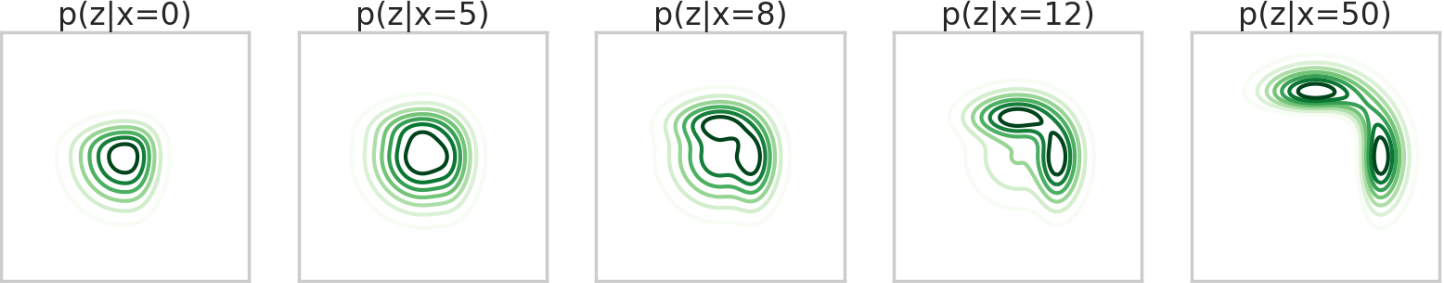
\includegraphics[width=\textwidth]{sprinklertrue.png}
\end{figure}
\begin{itemize}
\item Posterior is flexible and bimodal.
\item Use Gaussian KDE to find `true' KL divergence for $q_\phi(z|x=0,5,8,12,50)$.
\end{itemize}
\end{frame}
%\begin{frame}{Activation Function Experiment}{Experiment Outline}
%\begin{itemize}
%\item Common to use ReLU $g(x)=\max\{0,x\}$ as activation function for output layer of direct ratio estimator $r_\alpha(u)\simeq \frac{q(u)}{p(u)}$.
%\item Experiences `dying ReLU problem'.
%\item Linearity of ReLU activation causes imbalance between ratios in $(0,1)$ and $(1,\infty)$.
%\item We propose exponential activation function $g(x)=e^x$.
%\item Compare them with reverse KL divergence upper bound.
%\item Low training rate, high iterations.
%\end{itemize}
%\end{frame}
%\begin{frame}{Activation Function Experiment}{Results}
%\begin{table}[h]
%\scalebox{0.8}{
%\begin{tabular}{|c|c|c|}
%\hline
%Algorithm & Mean KL Divergence & Standard Deviation\\
%\hline
%Prior Contrastive - ReLU & 1.3807 & 0.0391\\
%\hline
%Prior Contrastive - Exp & 1.3265 & 0.0045\\
%\hline
%%Joint-Contrastive - ReLU & 1.6954 & 0.4337\\
%%\hline
%%Joint-Contrastive - Exp & 1.3397 & 0.0066\\
%%\hline
%\end{tabular}
%}
%\end{table}
%\begin{figure}[h]
%\scalebox{0.8}{
%\begin{subfigure}{\textwidth}
%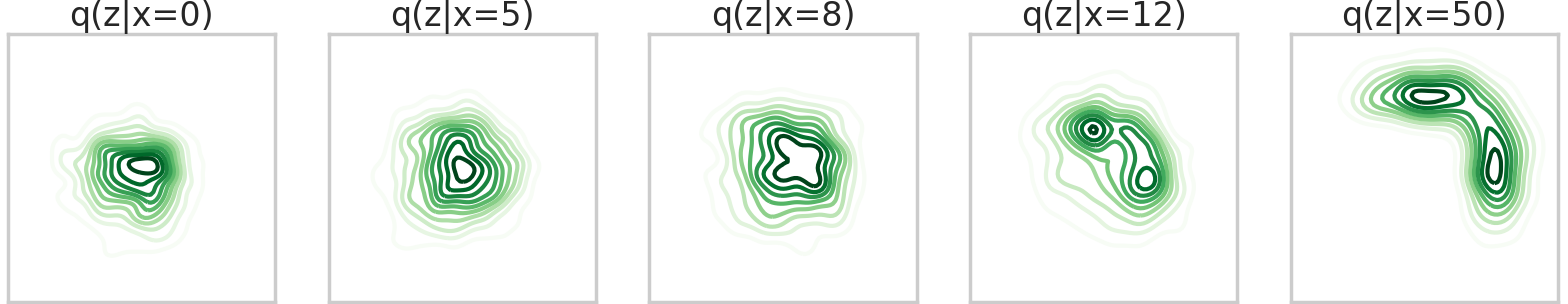
\includegraphics[width=\textwidth]{13288.png}
%\caption{Average KL Divergence of 1.3288}
%\end{subfigure}
%}
%\scalebox{0.8}{
%\begin{subfigure}{\textwidth}
%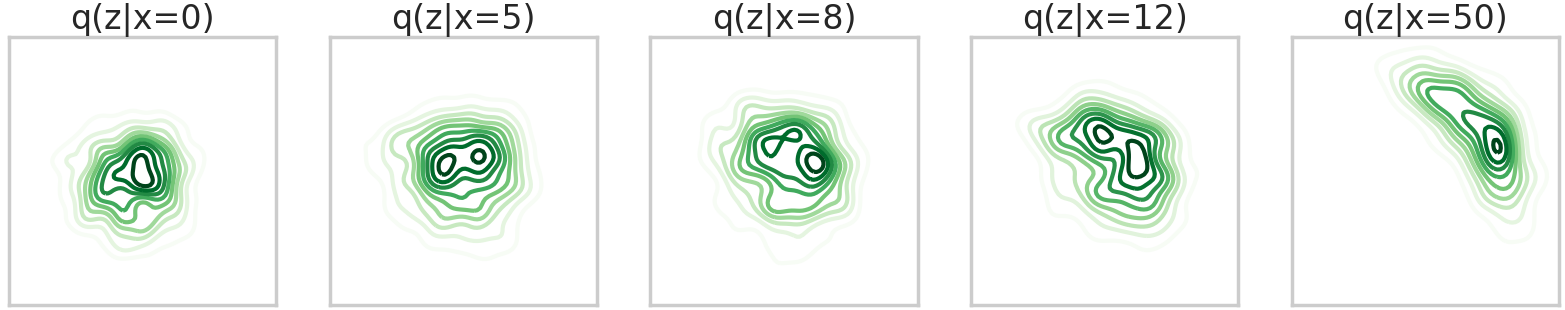
\includegraphics[width=\textwidth]{13963.png}
%\caption{Average KL Divergence of 1.3963}
%\end{subfigure}
%}
%\end{figure}
%\end{frame}
%\begin{frame}{Inference Experiment - Activation Function}{KL Divergence Plots}
%\begin{figure}
%\begin{subfigure}{0.49\textwidth}
%\includegraphics[width=\linewidth]{truklmins/PCKLvsPCKLEXP.png}
%\caption{True KL Divergence}
%\end{subfigure}
%\begin{subfigure}{0.49\textwidth}
%\includegraphics[width=\linewidth]{nelbos/PCKLvsPCKLEXP.png}
%\caption{NELBOs}
%\end{subfigure}
%\end{figure}
%\begin{itemize}
%\item Exponential output has smoother and faster convergence.
%\end{itemize}
%\end{frame}
%\begin{frame}{Inference Experiment - Activation Function}{NELBOs}
%\begin{figure}
%\begin{subfigure}{0.49\textwidth}
%\includegraphics[width=\linewidth]{nelbos/PCKLvsPCKLEXP.png}
%\caption{Prior-Contrastive}
%\end{subfigure}
%\begin{subfigure}{0.49\textwidth}
%\includegraphics[width=\linewidth]{nelbos/JCKLvsJCKLEXP.png}
%\caption{Joint-Contrastive}
%\end{subfigure}
%\end{figure}
%\begin{itemize}
%\item More stable NELBO estimation by exponential output.
%\item Variance of exponential output in joint-contrastive case increases over time.
%\end{itemize}
%\end{frame}
\begin{frame}{Undertrained Estimator Experiment}{Experiment Outline}
\begin{itemize}
\item In a previous experiment we found that all three estimator parametrisations lead to similar results when optimised effectively.
\vspace{0.5cm}
\item What if they are poorly optimised?
\vspace{0.5cm}
\item Training parameters:
\begin{itemize}
\item High posterior training rate.
\item Low estimator training rate.
\item Low estimator to posterior iteration ratio (11:1).
\end{itemize}
\end{itemize}
%\begin{figure}[h]
%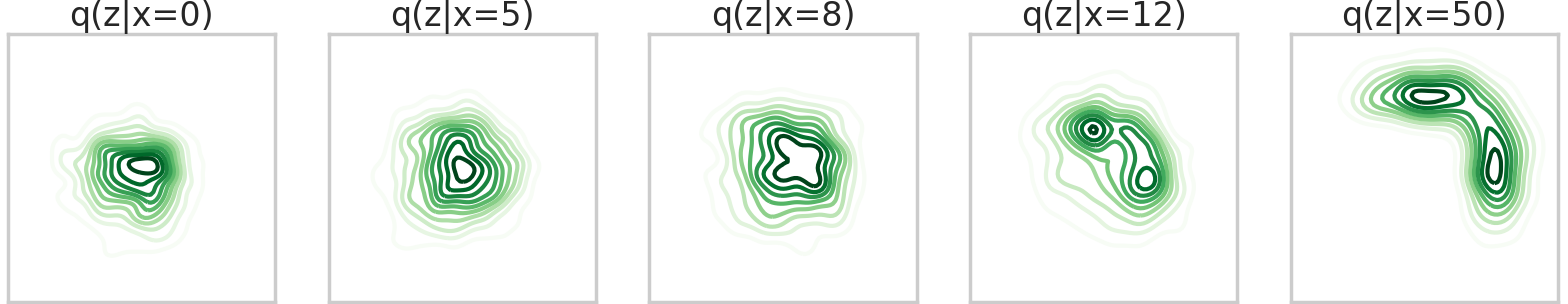
\includegraphics[width=\textwidth]{13288.png}
%\caption{`True' KL Divergence of 1.3288}
%\end{figure}
\end{frame}
%\begin{frame}{Optimal Estimator Experiment}{Results}
%\begin{table}[h]
%\scalebox{1.0}{
%\begin{tabular}{|c|c|c|}
%\hline
%Algorithm & Mean KL Divergence & Standard Deviation\\
%\hline
%JC Reverse KL - $D_\alpha(z,x)$ & \textbf{1.3416} & \textbf{0.0068}\\
%\hline
%JC Reverse KL - $r_\alpha(z,x)$ & \textbf{1.3397} & \textbf{0.0066}\\
%\hline
%JC Reverse KL - $T_\alpha(z,x)$ & \textbf{1.3446} & 0.0108\\
%\hline
%JC GAN - $D_\alpha(z,x)$ & 1.3648 & 0.0242\\
%\hline
%JC GAN - $r_\alpha(z,x)$ & 1.3657 & 0.0302\\
%\hline
%JC GAN - $T_\alpha(z,x)$ & 1.3670 & 0.0387\\
%\hline
%\end{tabular}
%}
%\end{table}
%\begin{itemize}
%
%\item No significant difference in convergence between estimators in each $f$-divergence.
%\item Reverse KL converged faster in joint-contrastive context.
%\end{itemize}
%\end{frame}
%\begin{frame}{Optimal Estimator Experiment}{Results}
%\begin{figure}
%\begin{subfigure}{\textwidth}
%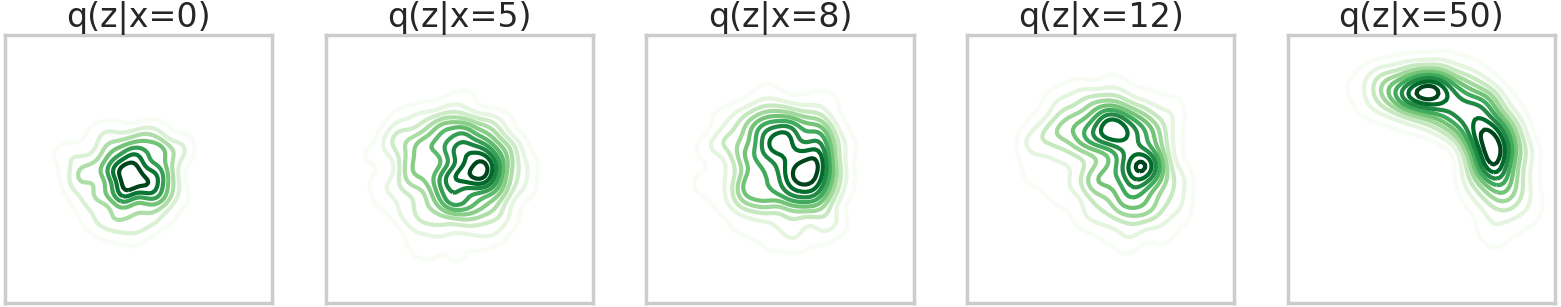
\includegraphics[width=\linewidth]{13474.png}
%\caption{`True' KL Divergence of 1.3474 (Reverse KL Algorithms)}
%\end{subfigure}
%\begin{subfigure}{\textwidth}
%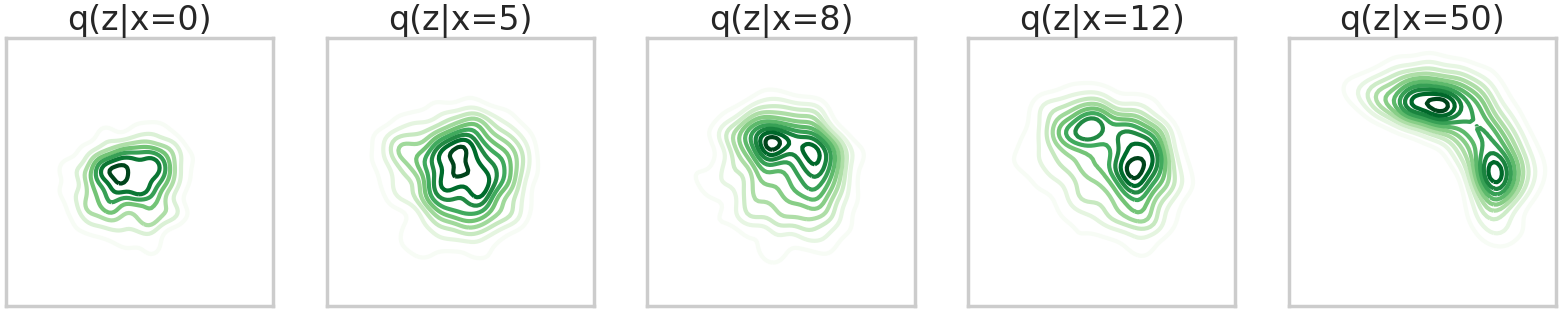
\includegraphics[width=\linewidth]{13623.png}
%\caption{`True' KL Divergence of 1.3623 (GAN Divergence Algorithms)}
%\end{subfigure}
%\end{figure}
%\end{frame}
%\section{Undertrained Estimator Experiment}
%\begin{frame}{Undertrained Estimator Experiment}{Experiment Outline}
%\begin{itemize}
%\item Estimators are similar when they are optimal but what if they are not optimal?
%\vspace{0.5cm}
%\item Same inference experiment again.
%\vspace{0.5cm}
%\item Significantly reduce amount of estimator training between posterior iterations.
%\vspace{0.5cm}
%\item Increased posterior training rate.
%\end{itemize}
%\end{frame}

\begin{frame}{Undertrained Estimator Experiment}{Results}
\begin{table}[h]
\scalebox{0.8}{
\begin{tabular}{|l|c|c|c|}
\hline
\multicolumn{2}{|l|}{Algorithm} & Mean KL Divergence & Standard Deviation\\
\hline
\multirow{3}{*}{Reverse KL} & $D_\alpha(z,x)$ & \textbf{1.3786} & \textbf{0.0286}\\
\cline{2-4}
 & $r_\alpha(z,x)$ & 1.3934 & 0.0410\\
 \cline{2-4}
 & $T_\alpha(z,x)$ & 1.4133 & 0.0597\\
\hline
\multirow{3}{*}{GAN} & $D_\alpha(z,x)$ & 1.4017 & \textbf{0.0286}\\
\cline{2-4}
 & $r_\alpha(z,x)$ & 1.4086 & 0.0555\\
 \cline{2-4}
 & $T_\alpha(z,x)$ & 1.4214 & 0.0518\\
\hline
\end{tabular}
}
\end{table}
\begin{figure}[h!]
\begin{subfigure}{0.3\textwidth}
\centering
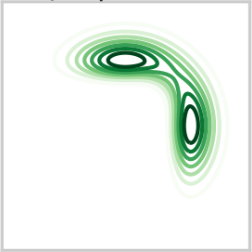
\includegraphics[width=0.5\linewidth]{sprinklertruea.png}
\caption*{\small True}
\end{subfigure}
\begin{subfigure}{0.3\textwidth}
\centering
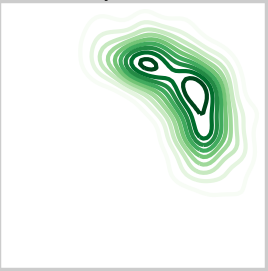
\includegraphics[width=0.5\linewidth]{13837a.png}
\caption*{\small Reverse KL}
\end{subfigure}
\begin{subfigure}{0.3\textwidth}
\centering
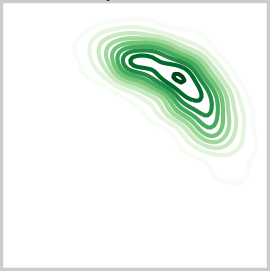
\includegraphics[width=0.5\linewidth]{14081a.png}
\caption*{\small GAN}
\end{subfigure}
\end{figure}
\begin{itemize}
\item Reverse KL divergence better than GAN divergence.
\item $D_\alpha(z,x)<r_\alpha(z,x)<T_\alpha(z,x)$
\end{itemize}
\end{frame}
\begin{frame}{Undertrained Estimator Experiment}{NELBO Plots}
\begin{figure}
\begin{subfigure}{0.49\textwidth}
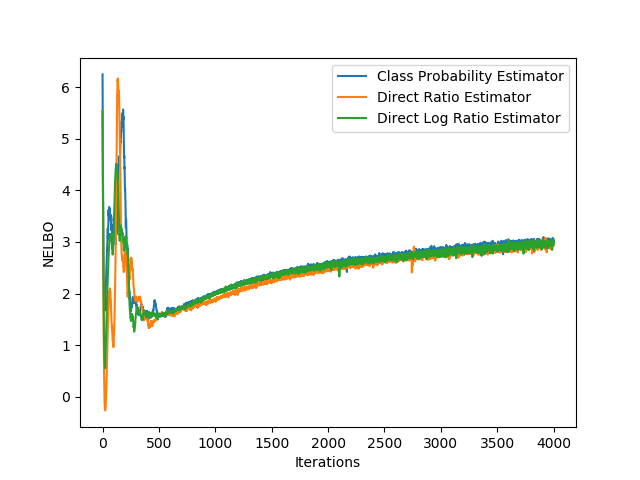
\includegraphics[width=\linewidth]{part2nelbos/JCKLDvsJCKLexpvsJCKLgudlog.png}
\caption{Reverse KL Divergence}
\end{subfigure}
\begin{subfigure}{0.49\textwidth}
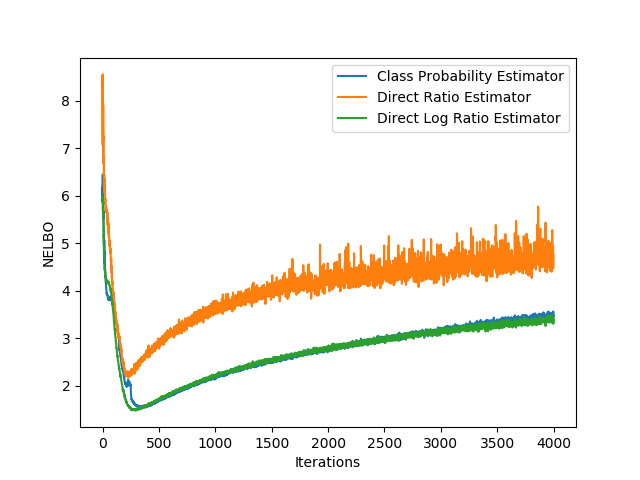
\includegraphics[width=\linewidth]{part2nelbos/JCADVvsJCADVexpvsJCADVgudlog.png}
\caption{GAN Divergence}
\end{subfigure}
\begin{itemize}
\vspace{0.3cm}
\item Reverse KL Divergence has initial instability.
\end{itemize}
\end{figure}
\end{frame}
\section{Autoencoder Experiment}
\begin{frame}{Autoencoder Experiment}{Autoencoders}
\begin{itemize}
\item Posterior $q_\phi(z|x)$ `compresses' data $x$ into $z$.
\item Likelihood $p_\theta(x|z)$ `reconstructs' data $\tilde{x}$ from $z$.
\end{itemize}
\begin{figure}[h]
  \centering
  \tikz{ %
    \node[latent] (x) {$\bm{x}$} ; %
    \node[det, right=of x] (q) {$q_\phi(z|x)$} ; %
    \node [latent, above=of x] (eps) {$\epsilon$} ;
    \node [latent, right=of q] (z) {$\bm{z}$} ;
    \node [det, right=of z] (p) {$p_\theta(x|z)$} ;
    \node [latent, right=of p] (pout) {$\tilde{\bm{x}}$} ;
    \edge {x} {q} ; %
    \edge {q} {z} ;
    \edge {eps} {q} ;
    \edge {z} {p} ;
    \edge {p} {pout} ;
  }
\end{figure}
\[\min_{\theta, \phi} \E_{q^*(x)}[\underbrace{-\mathbb{E}_{q_\phi(z|x)}[\log p_\theta(x|z)]}_{\text{Likelihood}}+\underbrace{KL(q_\phi(z|x)||p(z))}_{\text{Log Density Ratio}}]\]
\end{frame}
\begin{frame}{Autoencoder Experiment}{Autoencoders}
\begin{itemize}
\item Generate $z$ from $p(z)$.
\item Typically $p(z)$ is $\mathcal{N}(0,I)$.
\end{itemize}
\begin{figure}[h]
  \centering
  \tikz{ %
    \node [latent] (z) {$\bm{z}$} ;
    \node [det, right=of z] (p) {$p_\theta(x|z)$} ;
    \node [latent, right=of p] (pout) {$\tilde{\bm{x}}$} ;
    \edge {z} {p} ;
    \edge {p} {pout} ;
  }
\end{figure}
\end{frame}
\begin{frame}{Autoencoder Experiment}{Experiment Outline}
\begin{figure}
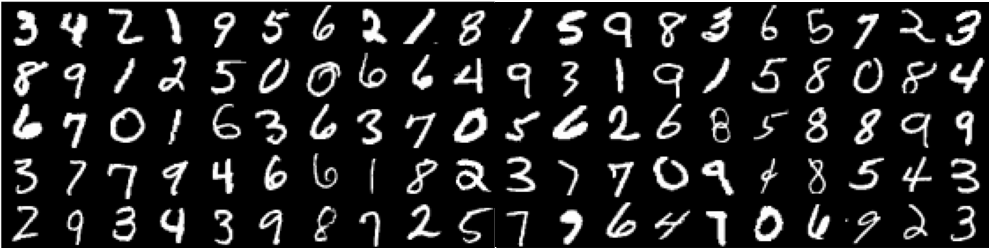
\includegraphics[width=\linewidth]{mnist-digits-small.png}
\end{figure}
\begin{itemize}
\item MNIST dataset - $28\times 28$ grey-scale images of handwritten digits
\vspace{0.3cm}
\item Again use undertrained estimator.
\vspace{0.3cm}
\item Use reconstruction error $\|x-\tilde{x}\|^2$ as metric.
\end{itemize}
\end{frame}
\begin{frame}{Generation Experiment}{Results - 20-dimensional latent space}
\begin{table}[h]
\scalebox{0.9}{
\begin{tabular}{|c|c|c|}
\hline
Algorithm & Mean Reconstruction Error & Standard Deviation\\
\hline
Reverse KL - $D_\alpha(z,x)$ & 0.0647 & 0.0019\\
\hline
GAN - $D_\alpha(z,x)$ & \textbf{0.0444} & \textbf{0.0017}\\
\hline

\end{tabular}
}
\end{table}
\begin{figure}
\begin{subfigure}{0.49\textwidth}
\centering

\includegraphics[width=0.5\linewidth]{064834a.png}
\caption*{Reverse KL}
\end{subfigure}
\begin{subfigure}{0.49\textwidth}
\centering
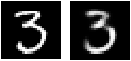
\includegraphics[width=0.5\linewidth]{044944a.png}
\caption*{GAN}
\end{subfigure}
\end{figure}
\begin{itemize}
\item Density ratios too big for direct ratio and log ratio estimators.
\item Exponential of $T_\alpha(z,x)$ taken in loss function.
\item $D_\alpha(z,x)$ ranges in $(0,1)$.
\end{itemize}

\end{frame}
\begin{frame}{Autoencoder Experiment}{NELBO plot}
\begin{figure}
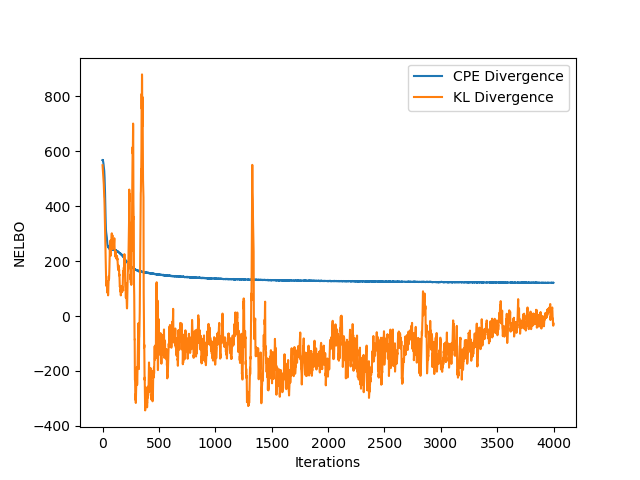
\includegraphics[width=0.49\linewidth]{part4nelbos/PCADVvsPCKLD.png}
\begin{itemize}
\vspace{0.3cm}
\item Reverse KL divergence fails to stabilise by the end of runtime.
\end{itemize}
\end{figure}

\end{frame}
%\begin{frame}{Blocks}
%\begin{block}{Block Title}
%You can also highlight sections of your presentation in a block, with it's own title
%\end{block}
%\begin{theorem}
%There are separate environments for theorems, examples, definitions and proofs.
%\end{theorem}
%\begin{example}
%Here is an example of an example block.
%\end{example}
%\end{frame}

% Placing a * after \section means it will not show in the
% outline or table of contents.3


\section*{Summary}

\begin{frame}{Summary}
  \begin{itemize}
  \item
    The class probability estimator $D_\alpha(u)\simeq\frac{q(u)}{q(u)+p(u)}$ is the `best' parametrisation as it can store the \alert{highest density ratios}.
  \item
    Reverse KL divergence upper bound may be \alert{unstable} but leads to \alert{faster convergence} when stable.
  \end{itemize}
  
  \begin{itemize}
  \item
    Future Research
    \begin{itemize}
    \item
      Still unclear exactly why reverse KL divergence is more unstable but more accurate when stable.
    \item
      Several more $f$-divergences exist which have unknown stability when undertrained.
    \item Alternate density ratio estimation algorithms e.g. denoisers, k-nearest neighbours
    \end{itemize}
  \end{itemize}
\end{frame}
%\begin{frame}{Cats}
%\begin{figure}
%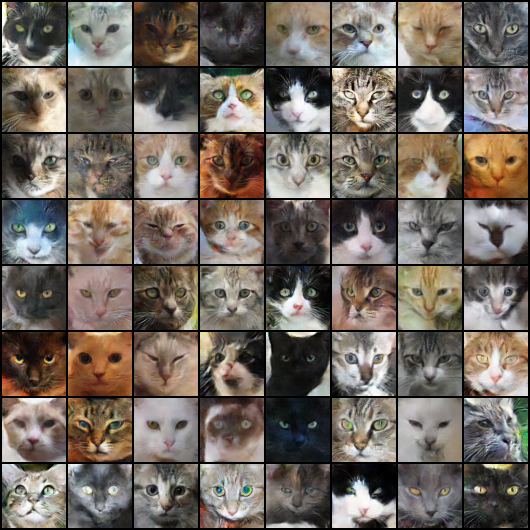
\includegraphics[scale=0.4]{cats.png}
%\end{figure}
%\end{frame}


% All of the following is optional and typically not needed. 
%\appendix
%\section<presentation>*{\appendixname}
%\subsection<presentation>*{For Further Reading}
%
\begin{frame}[allowframebreaks]
  \frametitle<presentation>{For Further Reading}
    
  \begin{thebibliography}{10}
    
  \beamertemplatebookbibitems
  % Start with overview books.

  \bibitem{Author1990}
    M.~Sugiyama, T.~Suzuki, T.~Kanamori
    \newblock {\em Density Ratio Estimation in Machine Learning}.
    \newblock Cambridge University Press, 2012.
 
    
  \beamertemplatearticlebibitems
  % Followed by interesting articles. Keep the list short. 
  \bibitem{blei}
    D.M.~Blei, A.~Kucukelbir, D.J.~McAuliffe
    \newblock Variational inference: A review for statisticians.
    \newblock {\em Journal of the American Statistical Association}, 112(518):859-877
    2017.
  \bibitem{Someone2000}
    F.~Huszar
    \newblock Variational Inference Using Implicit Distributions.
    \newblock {\em ArXiv e-prints},
    2017.
  \end{thebibliography}
\end{frame}

\end{document}


